% This file was created with tikzplotlib v0.10.1.post9.
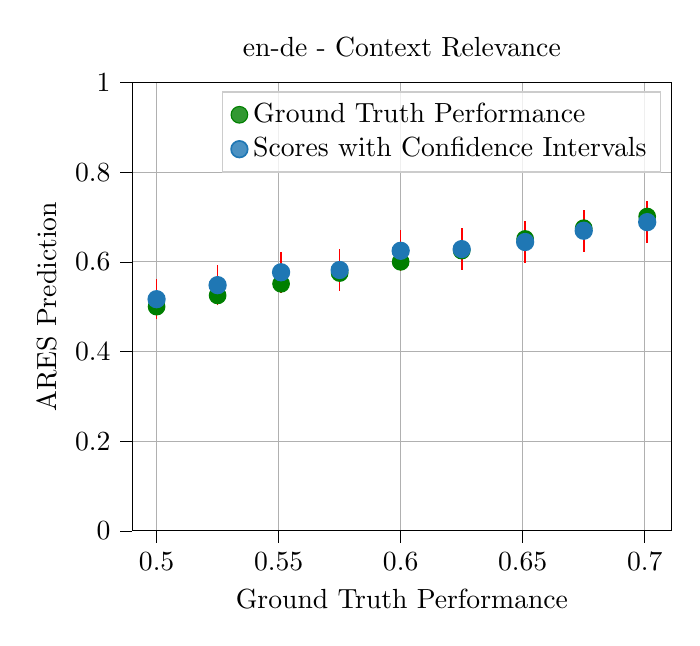
\begin{tikzpicture}

\definecolor{darkgrey176}{RGB}{176,176,176}
\definecolor{green01270}{RGB}{0,127,0}
\definecolor{lightgrey204}{RGB}{204,204,204}
\definecolor{steelblue31119180}{RGB}{31,119,180}

\begin{axis}[
legend cell align={left},
legend style={
  fill opacity=0.8,
  draw opacity=1,
  text opacity=1,
  draw=lightgrey204,
  mark options={mark size=3}
},
tick align=outside,
tick pos=left,
title={en-de - Context Relevance},
x grid style={darkgrey176},
xlabel={Ground Truth Performance},
xmajorgrids,
xmin=0.48995, xmax=0.71105,
xtick style={color=black},
y grid style={darkgrey176},
ylabel={ARES Prediction},
ymajorgrids,
ymin=0, ymax=1,
ytick style={color=black}
]
\addplot [draw=green01270, fill=green01270, mark size=3pt, mark=*, only marks]
table{%
x  y
0.5 0.5
0.525 0.525
0.551 0.551
0.575 0.575
0.6 0.6
0.625 0.625
0.651 0.651
0.675 0.675
0.701 0.701
};
\addlegendentry{Ground Truth Performance}
\path [draw=red, semithick]
(axis cs:0.5,0.472)
--(axis cs:0.5,0.561);

\path [draw=red, semithick]
(axis cs:0.525,0.503)
--(axis cs:0.525,0.593);

\path [draw=red, semithick]
(axis cs:0.551,0.531)
--(axis cs:0.551,0.622);

\path [draw=red, semithick]
(axis cs:0.575,0.536)
--(axis cs:0.575,0.628);

\path [draw=red, semithick]
(axis cs:0.6,0.579)
--(axis cs:0.6,0.671);

\path [draw=red, semithick]
(axis cs:0.625,0.582)
--(axis cs:0.625,0.675);

\path [draw=red, semithick]
(axis cs:0.651,0.598)
--(axis cs:0.651,0.691);

\path [draw=red, semithick]
(axis cs:0.675,0.623)
--(axis cs:0.675,0.716);

\path [draw=red, semithick]
(axis cs:0.701,0.642)
--(axis cs:0.701,0.735);

\addplot [semithick, steelblue31119180, mark=*, mark size=3, mark options={solid}, only marks]
table {%
0.5 0.516586826347305
0.525 0.547945492662474
0.551 0.576666666666667
0.575 0.581718331419824
0.6 0.624570858283433
0.625 0.628352059925094
0.651 0.644199134199134
0.675 0.669389038634322
0.701 0.688554778554779
};
\addlegendentry{Scores with Confidence Intervals}
\end{axis}

\end{tikzpicture}
